%%
%% This is file `sample-sigconf.tex',
%% generated with the docstrip utility.
%%
%% The original source files were:
%%
%% samples.dtx  (with options: `sigconf')
%% 
%% IMPORTANT NOTICE:
%% 
%% For the copyright see the source file.
%% 
%% Any modified versions of this file must be renamed
%% with new filenames distinct from sample-sigconf.tex.
%% 
%% For distribution of the original source see the terms
%% for copying and modification in the file samples.dtx.
%% 
%% This generated file may be distributed as long as the
%% original source files, as listed above, are part of the
%% same distribution. (The sources need not necessarily be
%% in the same archive or directory.)
%%
%% Commands for TeXCount
%TC:macro \cite [option:text,text]
%TC:macro \citep [option:text,text]
%TC:macro \citet [option:text,text]
%TC:envir table 0 1
%TC:envir table* 0 1
%TC:envir tabular [ignore] word
%TC:envir displaymath 0 word
%TC:envir math 0 word
%TC:envir comment 0 0
%%
%%
%% The first command in your LaTeX source must be the \documentclass command.
\documentclass[sigconf,anonymous,review]{acmart}
%% NOTE that a single column version may be required for 
%% submission and peer review. This can be done by changing
%% the \doucmentclass[...]{acmart} in this template to 
%% \documentclass[manuscript,screen]{acmart}
%% 
%% To ensure 100% compatibility, please check the white list of
%% approved LaTeX packages to be used with the Master Article Template at
%% https://www.acm.org/publications/taps/whitelist-of-latex-packages 
%% before creating your document. The white list page provides 
%% information on how to submit additional LaTeX packages for 
%% review and adoption.
%% Fonts used in the template cannot be substituted; margin 
%% adjustments are not allowed.
%%
%%
%% \BibTeX command to typeset BibTeX logo in the docs
\AtBeginDocument{%
  \providecommand\BibTeX{{%
    \normalfont B\kern-0.5em{\scshape i\kern-0.25em b}\kern-0.8em\TeX}}}

%% Rights management information.  This information is sent to you
%% when you complete the rights form.  These commands have SAMPLE
%% values in them; it is your responsibility as an author to replace
%% the commands and values with those provided to you when you
%% complete the rights form.
\setcopyright{acmcopyright}
\copyrightyear{2018}
\acmYear{2018}
\acmDOI{XXXXXXX.XXXXXXX}

%% These commands are for a PROCEEDINGS abstract or paper.
\acmConference[Conference acronym 'XX]{Make sure to enter the correct
  conference title from your rights confirmation emai}{June 03--05,
  2018}{Woodstock, NY}
%
%  Uncomment \acmBooktitle if th title of the proceedings is different
%  from ``Proceedings of ...''!
%
%\acmBooktitle{Woodstock '18: ACM Symposium on Neural Gaze Detection,
%  June 03--05, 2018, Woodstock, NY} 
\acmPrice{15.00}
\acmISBN{978-1-4503-XXXX-X/18/06}


%%
%% Submission ID.
%% Use this when submitting an article to a sponsored event. You'll
%% receive a unique submission ID from the organizers
%% of the event, and this ID should be used as the parameter to this command.
%%\acmSubmissionID{123-A56-BU3}

%%
%% The majority of ACM publications use numbered citations and
%% references.  The command \citestyle{authoryear} switches to the
%% "author year" style.
%%
%% If you are preparing content for an event
%% sponsored by ACM SIGGRAPH, you must use the "author year" style of
%% citations and references.
%% Uncommenting
%% the next command will enable that style.
%%\citestyle{acmauthoryear}

%%
%% end of the preamble, start of the body of the document source.
\usepackage{multirow}
\usepackage{cleveref}
\usepackage{color}
\newcommand{\KZ}[1]{\textcolor{blue}{Kenny: #1}}
\begin{document}

%%
%% The "title" command has an optional parameter,
%% allowing the author to define a "short title" to be used in page headers.
\title{CLAP: Contrastive Language-Audio Pre-training based on Large-Scale Synthetic Parallel Audio-Text Data}

%%
%% The "author" command and its associated commands are used to define
%% the authors and their affiliations.
%% Of note is the shared affiliation of the first two authors, and the
%% "authornote" and "authornotemark" commands
%% used to denote shared contribution to the research.
\author{Xuenan Xu}
% \authornote{Both authors contributed equally to this research.}
% \orcid{1234-5678-9012}
% \author{G.K.M. Tobin}
% \authornotemark[1]
% \email{webmaster@marysville-ohio.com}
\affiliation{%
  \institution{MoE Key Lab of Artificial Intelligence\\
  X-LANCE Lab\\
  Department of Computer Science and Engineering}
  \city{Shanghai}
  \country{China}
}
\email{wsntxxn@sjtu.edu.cn}

\author{Zhiling Zhang}
\affiliation{%
  \institution{The Th{\o}rv{\"a}ld Group}
  \streetaddress{1 Th{\o}rv{\"a}ld Circle}
  \city{Shanghai}
  \country{China}}
\email{larst@affiliation.org}

\author{Zelin Zhou}
\affiliation{%
  \institution{Inria Paris-Rocquencourt}
  \city{Shanghai}
  \country{China}
}

\author{Pingyue Zhang}
\affiliation{%
 \institution{MoE Key Lab of Artificial Intelligence\\
  X-LANCE Lab\\
  Department of Computer Science and Engineering}
 \city{Shanghai}
 \country{China}
}
\email{williamzhangsjtu@sjtu.edu.cn}

\author{Zeyu Xie}
\affiliation{%
 \institution{MoE Key Lab of Artificial Intelligence\\
  X-LANCE Lab\\
  Department of Computer Science and Engineering}
 \city{Shanghai}
 \country{China}
}
\email{zeyuxie29@gmail.com}


\author{Mengyue Wu}
\affiliation{%
  \institution{MoE Key Lab of Artificial Intelligence\\
  X-LANCE Lab\\
  Department of Computer Science and Engineering}
  \city{Shanghai}
  \country{China}
}
\email{mengyuewu@sjtu.edu.cn}

\author{Kenny Q. Zhu}
\affiliation{%
  \institution{Tsinghua University}
  \streetaddress{30 Shuangqing Rd}
  \city{Shanghai}
  \country{China}
}


%%
%% By default, the full list of authors will be used in the page
%% headers. Often, this list is too long, and will overlap
%% other information printed in the page headers. This command allows
%% the author to define a more concise list
%% of authors' names for this purpose.
\renewcommand{\shortauthors}{Trovato and Tobin, et al.}

%%
%% The abstract is a short summary of the work to be presented in the
%% article.
\begin{abstract}
%With the evolving deep learning models and large-scale datasets, multi-modal learning has witnessed rapid development in recent years.
%Multi-modal pretrained models have winteness rapid development thanks to the evolving deep learning models and large-scale datasets.
%However, audio-related multi-modal learning, especially audio-text pre-training, is still in a preliminary stage.
Compared with ample visual-text pre-training research, few works explore audio-text pre-training, which is mostly due to the lack of sufficient parallel audio-text data.
%Previous studies utilize data and pre-trained models from visual-related multi-modal research as supervision to learn audio-text correspondence.
%This may lead to noisy training data due to the probable mismatch between audio and visual content.
In this work, we utilize an audio-captioning based approach to expand parallel audio-text data with the large-scale audio event dataset AudioSet.
%using the most large-scale 
With the expanded synthetic 1.22M parallel audio-text pairs, we proposed Contrastive Language-Audio Pre-training (CLAP) where contrastive learning is used to pre-train an audio-text bi-encoder.
For the first time, we comprehensively demonstrate the performance of such a pre-trained bi-encoder audio-text model on a series of downstream audio-related tasks, including single modality tasks like audio classification and tagging, as well as cross-modal tasks consisting of audio-text retrieval and audio-based text generation. 
%which involves exclusively audio and textual modalities,
Experimental results indicate that our CLAP pre-trained on enlarged audio-text data achieves the state-of-the-art zero-shot classification performance on most datasets, which demonstrates the benefits of pre-training from a large amount of high-quality synthetic data.
\KZ{Perhaps no deed to mention this: The audio encoder also serves as an efficient pattern recognition model by fine-tuning it on audio-related tasks.}
%TODO without image? 带 image 的已经有一些了
%To our knowledge, this is by far the first general-purpose audio-text multimodal pre-training work achieving SOTA performance on a series of single- and cross-modal downstream tasks. 
% It can be further inferred that with appropriate method, pre-training bi-encoder models can benefit from large amount of high-quality synthetic data. 
\end{abstract}

%%
%% The code below is generated by the tool at http://dl.acm.org/ccs.cfm.
%% Please copy and paste the code instead of the example below.
%%
\begin{CCSXML}
<ccs2012>
   <concept>
       <concept_id>10010147.10010178</concept_id>
       <concept_desc>Computing methodologies~Artificial intelligence</concept_desc>
       <concept_significance>300</concept_significance>
       </concept>
   <concept>
       <concept_id>10010147.10010178.10010179</concept_id>
       <concept_desc>Computing methodologies~Natural language processing</concept_desc>
       <concept_significance>500</concept_significance>
       </concept>
 </ccs2012>
\end{CCSXML}

\ccsdesc[300]{Computing methodologies~Artificial intelligence}
\ccsdesc[500]{Computing methodologies~Natural language processing}

%%
%% Keywords. The author(s) should pick words that accurately describe
%% the work being presented. Separate the keywords with commas.
\keywords{multi-modal learning, contrastive learning, audio captioning, audio classification, zero-shot inference}

%% A "teaser" image appears between the author and affiliation
%% information and the body of the document, and typically spans the
%% page.
% \begin{teaserfigure}
%   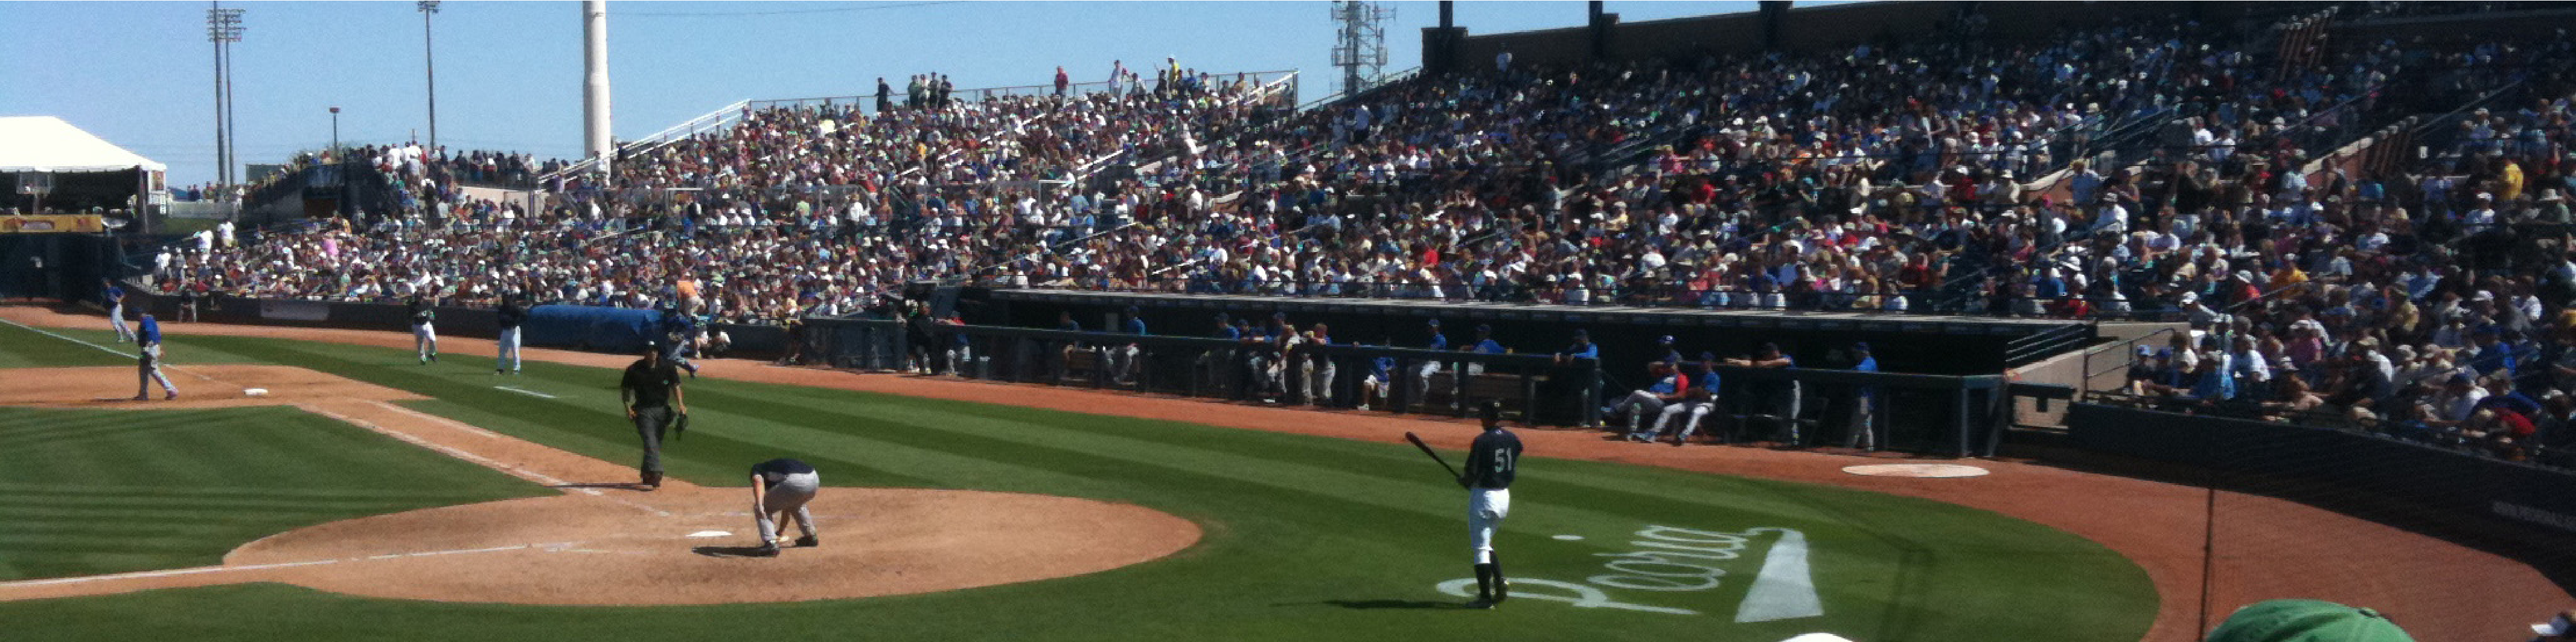
\includegraphics[width=\textwidth]{sampleteaser}
%   \caption{Seattle Mariners at Spring Training, 2010.}
%   \Description{Enjoying the baseball game from the third-base
%   seats. Ichiro Suzuki preparing to bat.}
%   \label{fig:teaser}
% \end{teaserfigure}

%%
%% This command processes the author and affiliation and title
%% information and builds the first part of the formatted document.
\maketitle

\section{Introduction}
\label{sec:intro}

Multi-modal machine learning has become increasingly popular since it mimics our experience of learning: we accept and handle information from different modalities. 
With the success of deep neural networks and large-scale datasets, we have witnessed rapid development of multi-modal learning in recent years.
Vision-language pre-training~\cite{chen2020uniter,li2020oscar,lu2019vilbert,su2019vl} using Transformer has pushed the state of the art (SOTA) on a wide range of cross-modal tasks, such as visual question answering (VQA)~\cite{antol2015vqa}, Image-Text Retrieval~\cite{lin2014microsoft}, visual commonsense reasoning (VCR)~\cite{zellers2019recognition}, etc.
In these works, a joint representation of vision and language modalities is learnt through pre-training on large-scale image-text datasets and then fine-tuned on specific downstream vision-language tasks.

Contrary to substantial efforts on vision-language pre-training, 
audio-related multi-modal learning, is still in its infancy. 
% especially audio-language pre-training, is still in a preliminary stage.
Although audio is an important modality, few works explore pre-training involving both audio and language.
The bottleneck of audio-language cross-modal learning lies in the 
scarcity of audio-text parallel data.
Compared with large-scale parallel image-text datasets such as COCO~\cite{lin2014microsoft} ($\sim$1.64M pairs), Visual Genome~\cite{krishna2017visual} ($\sim$5.06M pairs), and Conceptual Captions~\cite{sharma2018conceptual} ($\sim$ 12M pairs), current parallel audio-text datasets contain only about 100K pairs (see \Cref{subsec:real_datasets}).
The lack of large-scale parallel audio-text datasets may be attributed to the 
fact that not only the annotation of audio is much more costlier than 
that of image~\cite{zhang2021enriching} since it takes longer to listen
to the audio samples, but even the loosely coupled audio-text pairs are rare 
on the web~\cite{zhao2021connecting}.

%TODO 使用 image captioning data 的 work?
To alleviate the above problem of data scarcity, previous works on 
audio-text cross-modal learning mostly incorporate 
CLIP~\cite{radford2021learning}, a powerful model enabling image-text 
alignment, to facilitate audio-language representation learning.
The visual modality works as a pivot to connect audio and text since 
aligned video-audio data is abundant from most video clips.
However, mismatch between audio and visual modalities is commonly observed when detecting objects and events via sound and image.
For example, visible objects in videos do not necessarily make sounds while sounds may be produced by objects off-the-screen.
Such mismatch leads to noise in audio-visual and audio-text alignment based on visual pivoting, indicated by the limited improvement achieved by these studies~\cite{guzhov2021audioclip,zhao2021connecting,wu2021wav2clip}.%myw add refs

To overcome the data scarcity bottleneck while circumventing the data noise sourcing from other modalities, we propose an audio-captioning based approach to expand parallel audio-text data using AudioSet~\cite{gemmeke2017audio}, the most large-scale audio event dataset.
AudioSet contains only audio clips and corresponding audio event tags in the original dataset.
Based on the provided event tags, we train an AudioSet tag-guided audio captioning model.
With the guidance of human-annotated event tags, the generated captions are expected to be more related to the audio content. 
%captions generated by the model are more content-related to the audio in terms of sound events.
We thus create a large-scale synthetic parallel audio-text corpus containing 1.22M pairs.
Similar to CLIP, we perform contrastive language-audio pre-training (CLAP) on an audio-text bi-encoder, which consists of separate audio and text encoders.
The pre-training is comprised of two steps: 1) pre-training on the large-scale synthetic data; 2) further pre-training on real data to adapt to the real distribution.

After pre-training, CLAP can be further transferred to cross-modal and single-modality tasks.
For the first time, we present a comprehensive performance analysis of such a pure audio-text bi-encoder on a series of downstream tasks, including audio-text retrieval, audio captioning and audio classification.
Results show that significant achievements can be achieved by fine-tuning CLAP on a panel of tasks.
With the supervision of natural language, CLAP achieves SOTA zero-shot classification performance on most datasets.
By linear probing and fine-tuning the audio encoder of CLAP, we show that CLAP works as an efficient audio feature extractor which can be conveniently transferred to audio classification tasks of different domains.

The main contribution of this paper can be summarized as follows:
\begin{itemize}
    \item We propose an AudioSet tag-guided audio captioning based approach to generate large-scale synthetic audio-text data to facilitate audio-text pre-training.
    \item We perform the first pure audio-text contrastive pre-training paradigm based on the synthetic parallel data. The exclusion of CLIP from audio-text pre-training helps eliminate the noise induced by the visual modality.
    \item We validate the effect of pre-training by fine-tuning CLAP on cross-modal and single-modality tasks including classification, retrieval and generation. CLAP fine-tuning consistently outperforms the baseline trained from scratch.
    \item We achieve SOTA zero-shot classification performance on several datasets with the supervision of natural language.  
\end{itemize}


\section{Related Work}


\subsection{Vision-Language Pre-training}
The research on multi-modal pre-trained models initially thrives in the intersection of vision and language modality. 
% Due to the relatively low annotation cost and the abundant image-text pairs naturally occur on the Internet, there are rich data for vision-language pre-training like the annotated COCO dataset~\citep{lin2014microsoft} , Visual Genome~\citep{krishna2017visual}, and the online-collected Conceptual Captions \citep{sharma2018conceptual}. 
Vision-language pre-trained models generally handles three groups of tasks: understanding tasks like Classification, VQA and Visual Entailment, generation tasks like Image Captioning, and Image-Text Retrieval/Matching tasks.
Researchers have proposed different model structures that are specifically suitable for certain group(s) of tasks. 
Cross-Encoder models process multi-modal inputs in the same encoder to allow full interaction of the two modalities and thus are generally performing well on understanding tasks \citep{chen2020uniter,li2020oscar}. 
Bi-Encoder models encode the visual and textual inputs with different encoders to get separate embeddings  \citep{radford2021learning,jia2021scaling}.
Since the embeddings can be pre-computed and stored for query, they are favorable for efficient retrieval. 
Encoder-Decoder models encode single or both modalities in the encoder, and use a decoder for generation, which provides the capability for generation tasks \citep{wang2021simvlm,wang2022unifying}.
Our model mainly adopts the Bi-Encoder paradigm.
We exhibit that it can achieve competitive performance across all three groups of tasks.

For pre-training models, the data size has been shown to be vital for performance regardless of model structure and data quality. %TODO myw add ref
%Regardless of the model structure and data quality, the size of pre-training data has been shown to be vital for performance.
Experimental results from the bi-encoder model CLIP shows that its zero-shot image classification performance steadily increase with the number of images involved in pre-training.
Another bi-encoder ALIGN \citep{jia2021scaling} further scales up the pre-training data with noisy images from the web and shows that the models pre-trained on noisy data can still outperform those trained on higher-quality data given larger data size.
SimVLM \citep{wang2021simvlm}, an encoder-decoder model, also achieves great success in both understanding and generation tasks with the large pre-training data ALIGN.
Inspired by their findings, we propose to synthesize parallel audio-text data for audio-language pre-training, despite the potential noise in the synthetic data.


\subsection{Audio-Language Pre-training}
With the success of visual-language pre-training, a few recent works start to incorporate audio into multi-modal pre-training.
For instance, an audio encoder is added into CLIP with the contrastive learning paradigm.
%is widely adopted by adding an audio encoder into CLIP.
Large-scale video-text datasets are often utilized since the dataset provides visual-text alignment while audio-visual alignment is naturally available from the video data.
VATT~\cite{akbari2021vatt} and MMV~\cite{alayrac2020self} uses HowTo100M~\cite{miech2019howto100m} and AudioSet for pre-training.
The audio-text alignment is learnt implicitly through the pivot of visual modality.
They validate the effect of pre-training mainly on video action recognition and image classification tasks.
AudioCLIP~\cite{guzhov2021audioclip} performs the tri-modal contrastive learning explicitly by using AudioSet event tags as the corresponding text.
It focuses on transferring to image and audio classification tasks.
Wav2CLIP~\cite{wu2021wav2clip}, in contrast, does not incorporate text into pre-training.
It distills CLIP by pre-training on audio-visual alignment in VGGSound~\cite{chen2020vggsound}.
The learnt audio representation is evaluated on several downstream tasks.
Following these works, we adopt contrastive pre-training to learn audio-text cross-modal representation.

Compared with either textual AudioSet tags or video description, VIP$\sim$A$_\text{N}$T~\cite{zhao2021connecting} is proposed recently to curating audio-text pairs by providing natural language audio-focused description for audio clips.
CLIP with the prompt ``the sound of'' is utilized to retrieve captions from the current audio captioning corpus for AudioSet audio clips.
A frame of the corresponding video is used as the query.
In this way, large-scale parallel audio-text pairs are automatically curated using the visual pivot.
Audio-language pre-training without explicitly incorporating the visual modality is conducted on the curated parallel audio-text data.
They achieve competitive zero-shot audio-text retrieval and audio classification performance.
Inspired by VIP$\sim$A$_\text{N}$T, we generate large-scale parallel audio-text data based on AudioSet and audio captioning.


\subsection{Audio Event Recognition}
% sound event classification, audio tagging, audio captioning, audio retrieval
Audio event recognition is an emerging field which attracts increasing amount of attention recently.
It requires recognizing the rich information in the sounds surrounding us, including the acoustic scenes where we are and what events are present.
Audio event recognition contains various tasks like acoustic scene classification~\cite{mesaros2018multi}, audio tagging~\cite{gemmeke2017audio} and sound event detection~\cite{cakir2015polyphonic}.
In recent years, the release of Detection and Classification of Acoustic Scenes and Events (DCASE) challenges encourages the development of novel datasets, tasks and approaches.
The release of AudioSet is also a milestone for audio event recognition.
It contains 2.08M 10-second audio clips\footnote{Only 1.95M clips are available in this work since some videos are removed.} with 527 annotated sound events.
Robust audio representations can be learnt by pre-training a deep neural network on AudioSet.
Outstanding performance can be achieved by fine-tuning the pre-trained network on downstream classification tasks.
Besides AudioSet, datasets like VGGSound and FSD50K~\cite{fonseca2022fsd50k} are also released recently to facilitate further research.

More recently, audio captioning~\cite{drossos2017automated} is proposed.
Beyond audio event tags, a caption provides unconstrained natural language description of an audio clip.
Several datasets (see \Cref{subsec:real_datasets}) are proposed to enable audio captioning research.
Audio-text retrieval~\cite{oncescu21audio} is also proposed recently which requires retrieving audio signals using their textual descriptions and vice versa.
The audio-language pre-training in this work is conducted based on these audio-text datasets.
We evaluate the benefit of pre-training by fine-tuning CLAP on these audio event recognition and audio-text tasks.



\section{Data Preparation}
In this work, we use both currently available audio-text datasets and synthetic parallel audio-text data for pre-training.
We describe these datasets and synthetic audio-text data generation approach in this section. 

\subsection{Existing Audio-Text Datasets}
\label{subsec:real_datasets}

\begin{table}[ht]
    \centering
    \begin{tabular}{c||ccc|c|c}
    \toprule
    \multirow{2}{*}{Dataset} & \multicolumn{3}{c|}{\# Audio-text pairs} & \multirow{2}{*}{Avg \# words} & \multirow{2}{*}{Duration /h} \\
    \cline{2-4}
     & train & val & test & & \\
    \midrule
    %TODO replace with available data
    AudioCaps & 49501 & 2475 & 4820 & 8.80 & 127\\
    \hline
    Clotho & 19195 & 5225 & 5225 & 11.33 & 44\\
    \hline
    MACS & \multicolumn{3}{c|}{17275} & 9.25 & 11\\
    \midrule
    %TODO check statistics
    Total & 85971 & 7700 & 10045 & 9.60 & 182\\
    \bottomrule
    \end{tabular}
    \caption{Statistics of current English audio-text datasets.}
    \label{tab:real_datasets}
\end{table}

Current parallel audio-text datasets are from audio captioning, including AudioCaps~\cite{kim2019audiocaps}, Clotho~\cite{drossos2020clotho} and MACS~\cite{martin2021diversity}.
AudioCaps is a subset of AudioSet, containing about 50K audio clips.
Each audio clip in the training set has one caption annotation while five annotations are provided for audio clips in the validation and test set.
Clotho contains 5,929 audio clips with five caption annotations provided for each clip.
The audio data are collected from Freesound~\cite{font2013freesound} platform.
MACS is a recently released dataset built on TAU Urban Acoustic Scenes 2019 dataset containing 3,930 audio clips.
Each audio clip is annotated by several captions, ranging from two to five.
The dataset does not provide splits of training, validation or test.
A summary of these datasets is in \Cref{tab:real_datasets}.



\subsection{Data Synthesis by Audio Captioning}
\label{subsec:syn_data_generation}

\begin{figure}[ht]
    \centering
    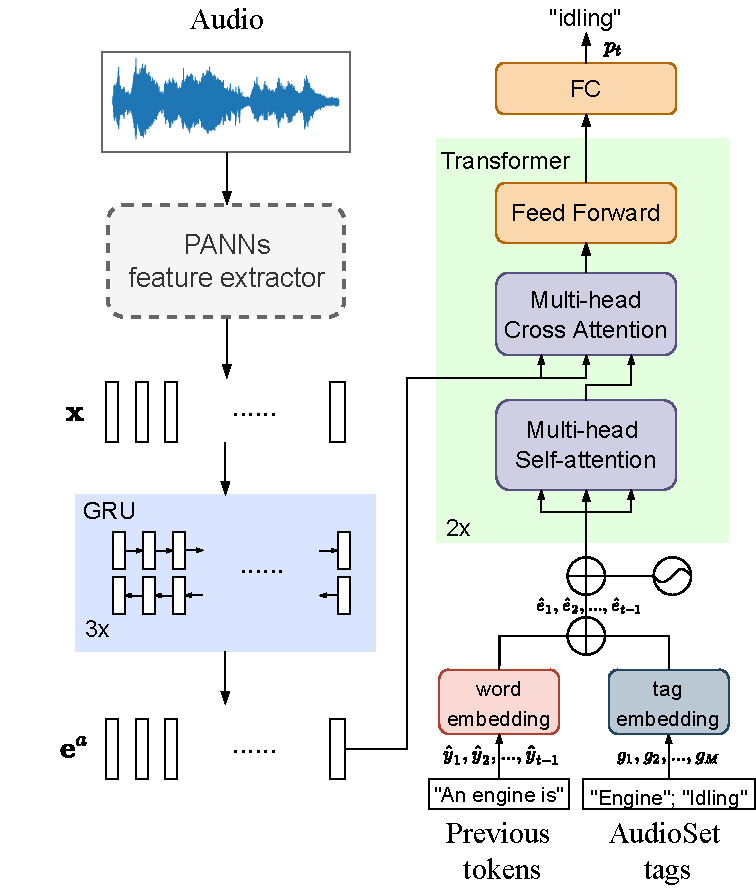
\includegraphics[width=\linewidth]{figs/tag_caption_model.pdf}
    \caption{The proposed audio captioning system with AudioSet tag guidance. The system generates caption based on both the input audio clip and the provided AudioSet tags.}
    \label{fig:tag_caption_model}
\end{figure}

%TODO why using both audio and AudioSet tags for parallel data generation?
Although about 100K audio-text pairs are available in current audio-text datasets, the dataset size is much smaller than image-text datasets (see \Cref{sec:intro}). %myw provide a number for image-text data size
%TODO xnx intro里有写,这里需要再放数字吗
However, large-scale audio event data are available from AudioSet. 
To leverage the large-scale audio-only data without caption description, we aim to generate captions for audio clips in AudioSet.
Since AudioCaps is a subset of AudioSet, we first train a captioning model on AudioCaps and then use it to generate parallel audio-text data from AudioSet.
\begin{figure*}[!htpb]
    \centering
    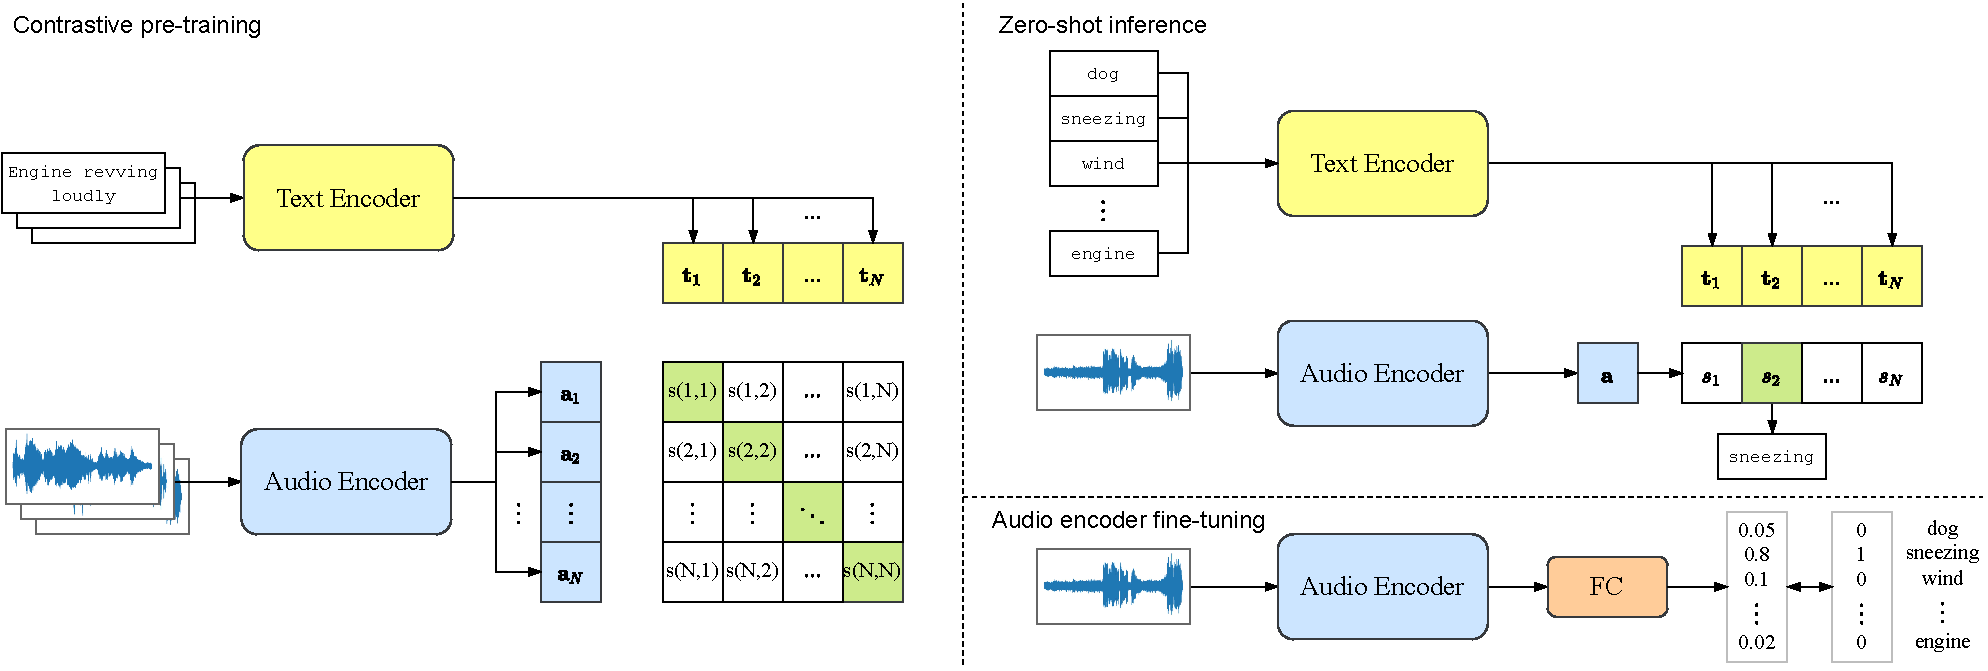
\includegraphics[width=\linewidth]{figs/CLAP.pdf}
    \caption{An overview of our proposed language-audio pre-training approach. Similar to CLIP, we first train an audio encoder and a text encoder jointly by contrastive learning. Then the pre-trained bi-encoder can be transferred to zero-shot classification. The pre-trained audio encoder can also be treated as a better feature extractor and be further fine-tuned on downstream tasks.}
    \label{fig:CLAP_framework}
\end{figure*}
Recent works tend to make use of supplementary information to guide captioning such as keyword~\cite{eren2020semantic} and similar captions~\cite{koizumi2020audio}).
However, these systems often suffer from poor prediction accuracy of supplementary information since the guidance can only be inferred from the input audio during inference.
In AudioSet, the label, consisting of audio event tags presented in the audio clip, serve as an effective guidance since it is available for all clips.
Therefore, to enhance the quality of generated captions, we incorporate the event tags into caption generation.
The model generates a caption conditioned on both the input audio and the hint from AudioSet tags.
The architecture is shown in \Cref{fig:tag_caption_model}.
It contains an audio encoder and a text decoder.
A sequence of audio features $\mathbf{x}$ is fed to the encoder and transformed into a sequence of high-level representations $\mathbf{e}^{a}$.
$$
    \mathbf{e}^{a} = \text{Encoder}(\mathbf{x})
$$
The decoder predicts the probability of each token at the time-step $t$ conditioned on partly decoded tokens $\{\hat{y}_n\}_{n=1}^{t-1}$, the provided AudioSet tags $\{{g}_m\}_{m=1}^{M}$ ($M$ is the number of tags) and $\mathbf{e}^{a}$:
$$
    p_t = \text{Decoder}(\mathbf{e}^{a}, \{\hat{e}_n\}_{n=1}^{t-1})
$$
$$
    \hat{e}_n = {e}_{n}^{w} + {e}^{g}
$$
$$
    {e}_{n}^{w}=\text{WE}(\hat{y}_n),
    \quad {e}^{g} = \frac{1}{M} \sum_{m=1}^{M}{\text{TE}(g_m)}
$$
where WE and TE denote word embedding and tag embedding layer which transform $\hat{y}_n$ and ${g}_m$ into fixed-dimensional vectors.
Starting from the special ``$<$BOS$>$'' token, the decoder auto-regressively predicts the next token until ``$<$EOS$>$'' is reached.

In this work, we utilize deep embeddings from PANNs, specifically the \textit{CNN14} variant, as the input audio feature $\mathbf{x}$.
The encoder is a three-layer bidirectional gated recurrent unit (GRU) following \cite{eren2020semantic} while the decoder is a two-layer Transformer with the final fully connected (FC) layer.
The captioning system is trained by word-level cross entropy (CE) loss:
$$
    \mathcal{L} = \sum_{t=1}^T-\log\left(p_t(y_t)\right)
$$
where $y_t$ is the ground truth token at the time-step $t$.

After training the AudioSet tag-guided captioning model, we use it to generate captions for large-scale AudioSet audio clips.
However, the data distribution of AudioCaps is different from AudioSet since audio clips with specific event tags are excluded during the construction process of AudioCaps~\cite{kim2019audiocaps}.
To circumvent the distribution bias problem, we exclude audio clips with tags that never appear in AudioCaps, with about 1.22M audio clips left.
One caption is generated for each audio clip using the enhanced captioning model, resulting in about 1.22M audio-text pairs.
We use this large-scale synthetic parallel audio-text data for pre-training.

\section{Audio-Text Pretraining Framework}

In this section, we describe the proposed framework of contrastive audio-text bi-modal representation learning from audio-text pairs.
The framework consists of an audio encoder and a text encoder for the two modalities.
As \Cref{fig:CLAP_framework} shows, the model is first pre-trained by contrastive learning.
Then the pre-trained model is used for zero-shot inference by calculating the similarity scores between the audio clip and all textual labels.
The audio encoder can be further fine-tuned on downstream tasks to boost performance.

We first illustrate the contrastive pre-training approach.
Then the architectures of the two encoders are introduced respectively.

\subsection{Contrastive Language-Audio Pre-training}
Similar to CLIP, the proposed contrastive learning approach learns the correspondence between the text content and the audio events in an arbitrary audio-text pair.
% 体现在 audio 和 text embedding 的 similarity 上
For an audio clip $\mathcal{A}$ and a sentence $\mathcal{T}$, the audio and text encoders $\text{Enc}_A$ and $\text{Enc}_T$ transform them into two embeddings $\mathbf{a}$ and $\mathbf{t}$ respectively.
A multi-modal embedding space is learned by maximizing the similarity between $\mathbf{a}$ and $\mathbf{t}$ of matched audio-text pairs and minimizing that of mismatched pairs.
Following CLIP, the training objective is to minimize the InfoNCE loss~\cite{van2018representation}.
Given a minibatch of $N$ audio-text pairs $(\mathcal{A}_1, \mathcal{T}_1), (\mathcal{A}_2, \mathcal{T}_2),\ldots, (\mathcal{A}_N, \mathcal{T}_N)$, their embeddings are calculated:
\begin{align*}
\begin{split}
   \mathbf{a}_i &= \text{Enc}_A (\mathcal{A}_i)\\
    \mathbf{t}_i &= \text{Enc}_T (\mathcal{T}_i)
\end{split}
\end{align*}
The training loss is a symmetric cross entropy loss between the predicted cosine similarity scores and the ground truth pairing labels:
\begin{align*}
    \begin{split}
        &s(i, j) = \frac{\mathbf{a}_i\cdot\mathbf{t}_j^{\mathrm{T}}}{
        \Vert \mathbf{a}_i \Vert \cdot \Vert \mathbf{t}_j \Vert
        }\\
        &\mathcal{L}_i^{A \rightarrow T} = -\log \frac{exp\left(s(i, i\right) / \tau )}{\sum_{j=1}^N exp(s\left(i, j\right) / \tau)}\\
        &\mathcal{L}_i^{T \rightarrow A} = -\log \frac{exp\left(s(i, i\right) / \tau )}{\sum_{j=1}^N exp(s\left(j, i\right) / \tau)}\\
        &\mathcal{L} = \frac{1}{N}\sum_{i=1}^N(\mathcal{L}_i^{A \rightarrow T} + \mathcal{L}_i^{T \rightarrow A})
    \end{split}
\end{align*}
where $\tau$ is the temperature optimized jointly with $\text{Enc}_A$ and $\text{Enc}_T$.


\subsection{Audio Encoder}
Similar to the feature extractor in \Cref{subsec:syn_data_generation}, we use the pre-trained CNN14 from PANNs~\citep{kong2020panns} as $\text{Enc}_A$ instead of training the model from scratch.
Time-frequency representation Log Mel Spectrogram (LMS) is extracted from the input audio and fed to 12 convolution blocks. %, where each block contains a $3\times3$ convolution layer, a batch normalization layer and a ReLU activation.
$2\times2$ max pooling is done between every two blocks.
After the convolution blocks, the audio embedding \textbf{a} is obtained by a global pooling on the feature map and transformation through a fully-connected layer. 
% The CNN14 is trained on AudioSet and achieves promising audio tagging performance.
% It also shows superior performance after transferred to other audio-related tasks.
Although Transformer-based models are applied for audio classification recently~\cite{gong2021audio} and achieves better performance than convolutional neural networks (CNN), it works on a sequence of patch embeddings without sub-sampling, resulting in high memory demand.
Therefore, we adopt the pre-trained CNN14 to enable a larger minibatch size for training.

\subsection{Text Encoder}
For the text encoding part, we utilize BERT to transform $\mathcal{T}$ into $\mathbf{t}$.
It is a deep Transformer pre-trained on large-scale corpus, including BooksCorpus and English Wikipedia, by self-supervised learning.
Due to its powerful capability to extract representations with contextual semantics, BERT has exhibited superior performance on a series of language understanding tasks~\cite{devlin2019bert}. %myw add ref
In this work, we employ BERT$_\text{MEDIUM}$~\cite{turc2019well} as Enc$_T$ for better computation efficiency and lower memory requirements.
It consists of eight Transformer layers with a hidden embedding size of 512.


\section{Experimental Setup}
In this section, we first present our experimental setup in training the audio captioning model to synthetic parallel audio-text data generation.
Then the CLAP pre-training, fine-tuning and evaluation procedures are described in detail.

\subsection{AudioSet Tag-Guided Audio Captioning Model Training}
\label{subsec:syn_data_generation_setup}

% Special tokens ``$<$BOS$>$'' and ``$<$EOS$>$'' are appended before and after the original caption for training the captioning model.
The AudioSet tag-guided captioning model is trained on AudioCaps for 25 epochs with a batch size of 64.
The learning rate linearly warms up to $5\times10^{-4}$ and then exponentially decays to $5\times10^{-7}$ until the end of training.
Scheduled sampling~\cite{bengio2015scheduled} and label smoothing~\cite{szegedy2016rethinking} are used for regularization.
We use stochastic weight average~\cite{izmailov2018averaging} by averaging the last five checkpoints as the final model.
For inference on AudioSet audio clips, we use beam search with a beam size of three.

\subsection{CLAP Pre-training}
The contrastive pre-training consists two steps.
First, the model is pre-trained on large-scale synthetic parallel audio-text data mentioned in \Cref{subsec:syn_data_generation_setup}.
% TODO audio and text pre-process
% PANNs, tokenizer max_length = 30
We use a batch size of 128 and train the model for 200K iterations.
About 1,200 audio-text pairs are randomly selected from the synthetic data to form a separate validation set.
The model is validated every 500 iterations on the validation set.
% TODO validation metric: mean of a2t and t2a R1/R5/R10?
We use the Adam optimizer with the maximum learning rate of $1\times10^{-4}$.
The learning rate is decayed by a cosine scheduler~\cite{loshchilov2016sgdr} with linear warm up in the first 10k iterations.

After pre-training on the synthetic data, we further pre-train the model on the real data.
The model with the best performance on the synthetic validation set is used to initialize parameters for this step.
Since there is a gap between the quality of real and synthetic data, the second pre-training step is adopted to alleviate the bias caused by synthetic data.
We use the combination of all training sets of real audio-text data introduced in \Cref{subsec:real_datasets} for training.
The training setup is similar to the first step with several modifications on hyper-parameters.
The total training iterations and warm up iterations are 15000 and 750 while the model is validated every 750 iterations.
The bi-encoder trained after this step is referred to as CLAP.

\subsection{Downstream Tasks}

\begin{table}[ht]
    \centering
    \begin{tabular}{cccc}
    \toprule
    Task & Dataset & \# Audio clips & Metric \\
    \midrule
    Audio-text & AudioCaps & 50K & \multirow{2}{*}{R@K} \\
    Retrieval & Clotho & 6K & \\
    \hline
    Audio & AudioCaps & 50K & COCO \&  \\
    Captioning & Clotho & 6K & FENSE \\
    \hline
     & ESC50 & 2K & \multirow{4}{*}{Accuracy}\\
    Audio & UrbanSound8K & 8K & \\
    Classification & TAU2019 & 14K & \\
     & VGGSound & 192K & \\
    \hline
    Audio & FSD50K & 50K & \multirow{2}{*}{mAP}\\
    Tagging & AudioSet & 1.93M & \\
    \bottomrule
    \end{tabular}
    \caption{A summary of downstream cross-modal and single-modality tasks. TAU2019 is the acoustic scene dataset from DCASE2019 challenge task1A.}
    \label{tab:task_summary}
\end{table}

The pre-trained CLAP can be transferred to a series of downstream tasks, which is summarized in \Cref{tab:task_summary}, including both cross-modal tasks and single-modality tasks.

Cross-modal audio-text tasks include audio-text retrieval and audio captioning.
For audio-text retrieval, we use recall at K (R@K) as the evaluation metric.
Standard COCO evaluation metrics from image captioning are used to evaluate audio captioning performance.
Besides, we also incorporate recently proposed FENSE~\cite{zhou2021can} into evaluation for its higher correlation with human judgments.

Single-modality tasks include single-label (classification) and multi-label (tagging) audio classification.
Accuracy and mean average precision (mAP) are used for evaluation.
We include several datasets with the size ranging from 2K to 1.93M for comparison with previous works.
%TODO why not including AudioSet? awkward thing: not enough time to train and the labels are not very correct

\subsection{Zero-shot Classification}
With the pre-trained CLAP, we can perform zero-shot classification.
% We use the prompt ``Sound of'' to help inference.
If a textual label contains ``\_'', we replace ``\_'' with a blank.
% Then the prompt ``Sound of'' is prepended to these words for inference.
CLAP calculates the similarity scores between a given audio clip and all these textual labels.
These scores are treated as the predicted probability of each audio event for evaluation.

\subsection{Fine-tuning}

\subsubsection{Audio-text Retrieval}
The fine-tuning on audio-text retrieval tasks uses almost the same configuration as the pre-training step.
For both AudioCaps and Clotho, we fine-tune the pre-trained bi-encoder model for 20 epochs using the InfoNCE loss with a batch size of 128.
The learning rate linearly warms up to the maximum value in the first epoch.
The maximum learning rate for AudioCaps and Clotho are $5\times10^{-5}$ and $2\times10^{-6}$, respectively.

\subsubsection{Audio Captioning}
The audio captioning system is similar to the model in \Cref{subsec:syn_data_generation} except 1) the audio feature is extracted by CLAP instead of PANNs; 2) the system does not receive guidance from AudioSet tags.
For both AudioCaps and Clotho, the training and inference configuration follows \Cref{subsec:syn_data_generation_setup}.


\subsubsection{Audio Classification and Tagging}
For single-modality tasks, we further fine-tune the pre-trained audio encoder $\text{Enc}_A$.
An extra fully-connected (FC) layer is added to $\text{Enc}_A$ for classification.
We perform two types of fine-tuning: linear probing and fine-tuning the whole $\text{Enc}_A$.
For linear probing, $\text{Enc}_A$ is used as a feature extractor and only the final FC layer is trained while no parameters are frozen in the second setting.
%TODO batch size / learning rate / epochs ?
Cross entropy loss and binary cross entropy loss are used for classification and tagging training respectively.



\section{Results}
In this section, the performance of CLAP is presented comprehensively.
We first evaluate the quality of synthetic parallel audio-text data.
Then for both cross-modal and single-modality downstream tasks, we reveal the influence of pre-training.
For single-modality tasks, transferring is done by zero-shot classification and fine-tuning $\text{Enc}_A$.

\subsection{Benefits of Synthetic Parallel Audio-text Data}

\begin{table}[ht]
    \begin{tabular}{c|cccccc}
    \toprule
    & $\text{B}_4$ & R & M & C & S & F\\
    \midrule
    System & 26.4 & 49.0 & 24.5 & 80.4 & 21.0 & 62.5\\
    Human & 29.0 & 49.5 & 28.8 & 90.8 & 28.8 & 68.0\\
    \bottomrule
    \end{tabular}
    \label{tab:syn_data_quality}
    \caption{The comparison of synthetic parallel audio-text data and real data in terms of audio captioning performance. Metrics include $\text{BLEU}_4$ ($\text{B}_4$), $\text{ROUGE}_\text{L}$ (R), METEOR (M), CIDEr (C), SPICE (S) and FENSE (F).}
\end{table}

\begin{table*}[ht]
    \centering
    \begin{tabular}{c||cccccc||cccccc}
    \toprule
    \multirow{3}{*}{Training Data} & \multicolumn{6}{c||}{AudioCaps} & \multicolumn{6}{c}{Clotho} \\
    \cline{2-13}
     & \multicolumn{3}{c}{Audio $\Rightarrow$ Text} & \multicolumn{3}{c||}{Text $\Rightarrow$ Audio} & \multicolumn{3}{c}{Audio $\Rightarrow$ Text} & \multicolumn{3}{c}{Text $\Rightarrow$ Audio} \\
     & R@1 & R@5 & R@10 & R@1 & R@5 & R@10 & R@1  & R@5 & R@10 & R@1 & R@5 & R@10\\
    \midrule
    synthetic (1.22M) & 32.6 & 62.9 & 76.7 & 23.5 & 54.3 & 68.4 & 7.6 & 22.0
 & 31.5 & 5.6 & 15.8 & 23.8\\
    Curated AC (1.08M)~\cite{zhao2021connecting} & 15.2 & - & 52.9 & 9.9 & - & 45.6 & 7.1 & - & 30.7 & 6.7 & - & 29.1\\
    \midrule
    real & 40.0 & 72.9 & 84.9 & 33.7 & 69.3 & 82.1 & 18.5 & 42.2 & 54.4 & 13.3 & 34.4 & 48.0\\
    synthetic $\rightarrow$ real (CLAP) & 44.2 & 77.5 & 87.4 & 35.2 & 71.3 & 84.3 & 18.1 & 40.1 & 52.5 & 12.4 & 34.0 & 47.3\\
    \bottomrule
    \end{tabular}
     \caption{Audio-text retrieval performance of pre-trained models.}
    \label{tab:pre_train_effects}
\end{table*}

\begin{table*}[ht]
    \centering
    \begin{tabular}{c||cccccc||cccccc}
    \toprule
    \multirow{3}{*}{Model} & \multicolumn{6}{c||}{AudioCaps} & \multicolumn{6}{c}{Clotho} \\
    \cline{2-13}
     & \multicolumn{3}{c}{Audio $\Rightarrow$ Text} & \multicolumn{3}{c||}{Text $\Rightarrow$ Audio} & \multicolumn{3}{c}{Audio $\Rightarrow$ Text} & \multicolumn{3}{c}{Text $\Rightarrow$ Audio} \\
     & R@1 & R@5 & R@10 & R@1 & R@5 & R@10 & R@1  & R@5 & R@10 & R@1 & R@5 & R@10\\
    \midrule
    from scratch & 38.6 & 74.3 & 86.0 & 33.4 & 68.8 & 82.2 & 13.6 & 34.4 & 46.1 & 11.5 & 32.2 & 45.0\\
    fine-tune from CLAP & 47.4 & 78.1 & 87.6 & 38.0 & 72.9 & 84.5 & 18.4 & 38.5 & 53.4 & 14.2 & 36.6 & 49.6\\
    \bottomrule
    \end{tabular}
     \caption{A comparison of audio-text retrieval performance between the model trained from scratch and that fine-tuned with CLAP initialization.}
    \label{tab:retrieval_finetune}
\end{table*}

\begin{table*}[ht]
    \centering
    \begin{tabular}{c||cccccc||cccccc}
    \toprule
    \multirow{2}{*}{Audio Feature} & \multicolumn{6}{c||}{AudioCaps} & \multicolumn{6}{c}{Clotho} \\
    \cline{2-13}
     & $\text{B}_4$ & R & M & C & S & F & $\text{B}_4$ & R & M & C & S & F\\
    \midrule
    PANNs & 27.1 & 49.7 & 24.4 & 71.6 & 18.1 & 60.1 & 16.2 & 37.9 & 17.6 & 40.4 & 12.2 & 44.1\\
    CLAP  & 27.1 & 49.6 & 24.8 & 73.2 & 18.6 & 61.1 & 16.2 & 37.6 & 17.8 & 41.1 & 12.8 & 44.9\\
    \bottomrule
    \end{tabular}
     \caption{A comparison of audio captioning performance between using audio features extracted from PANNs and CLAP.}
    \label{tab:caption_finetune}
\end{table*}


The quality of synthetic data is first evaluated in terms of captioning performance.
We compare the performance of synthetic captions and human-annotated captions on AudioCaps test set.
Since human annotations are used both as the candidate to be evaluated and the reference, we use a round-robin evaluation schedule.
Specifically, in each round we exclude one reference annotation and evaluate the caption based on the left four annotations.
The five scores are averaged as the performance indicator.
\Cref{tab:syn_data_quality} shows the comparison.
Metrics reveal that the synthetic data performance is close to human annotations.
\KZ{Any explanation why the synthetic data does better with B/R/M than
C/S/F?}
With the guidance of AudioSet tags, the captioning model is capable of generating high-quality parallel audio-text data based on AudioSet.
% Though without any doubt there is a gap between real and synthetic data, these results indicate that the synthetic data are of high quality.

Then we conduct the pre-training of the bi-encoder model on synthetic parallel audio-text data.
The results are shown in the upper half of \Cref{tab:pre_train_effects}.
For comparison, we include the curated audio-focused captions (AC) from VIP$\sim$A$_\text{N}$T~\cite{zhao2021connecting}, which uses CLIP and the prompt ``the sound of'' to retrieve captions from AudioCaps and Clotho training corpus.
The two synthetic datasets share a similar size (1.22M and 1.08M).
Results indicate that the model trained on our synthetic data significantly outperforms VIP$\sim$A$_\text{N}$T except for text to audio retrieval on Clotho.
The inferior performance of pre-training on curated AC indicates that using the visual modality as a pivot between audio and text leads to noisy data.
The noise may come from the the mismatch between audio and visual modalities, 
explained in \Cref{sec:intro}.
Although the comparison is not fair since curated AC do not use audio-text alignments which we use to train the captioning model, our focus is that generating captions directly from audio and AudioSet tags eliminate the noise induced by the visual modality.
Note that Clotho captions are also used to curate audio-text data in VIP$\sim$A$_\text{N}$T while we only use AudioCaps to train the captioning model.
The model trained on our synthetic data may suffer from the distribution difference between the two datasets when evaluated on Clotho.

After the second pre-training stage, the model learns the distribution of real data and achieves good performance on both datasets, especially on Clotho.
To validate the effectiveness of synthetic parallel audio-text data, 
we also train an bi-encoder on real data from scratch.
\KZ{What is ``real'' in the table? is it the same as the curated AC in the upper
half?}
The comparison is given in the lower half of \Cref{tab:pre_train_effects}.
Pre-training on synthetic data achieves significant performance improvement on AudioCaps while the performance on Clotho is comparable with the model trained from scratch, indicating the benefit of large-scale pre-training.
\KZ{It seems that the results on Clotho in the lower half is not that good,
explain?}

\begin{table*}[ht]
    \centering
    \begin{tabular}{cc||cccccc}
    \toprule
     & Model & ESC50 & UrbanSound8K & TAU2019 & VGGSound (mAP) & FSD50K & AudioSet\\
    \midrule
     %TODO check really SOTA?
     & SOTA & 95.9 & 89.5 & 85.1 & 52.5 & 56.7 & 45.9\\
    \midrule
    %TODO wav2clip zero-shot asc2019
    \multirow{4}{*}{Zero-shot} & AudioCLIP & 69.4 & 68.8 & - & - & - & -\\
     & Wav2CLIP & 41.4 & 40.4 & - & - (10.0) & 3.0 & - \\
     & VIP$\sim$A$_\text{N}$T & 69.2 & 71.7 & - & - & - & 13.3\\
     & CLAP & 80.6 & 77.3 & 32.2 & 14.9 (13.5) & 31.3 & 10.5\\
    \midrule
    \multirow{2}{*}{Linear probing} & PANNs & 90.8 & 82.5 & 58.9 & 41.1 & 29.8 & - \\
     & CLAP & 94.4 & 86.1 & 63.2 & 43.6 & 33.3 & 38.8\\
    \midrule
    \multirow{2}{*}{Fine-tuning} & PANNs & 94.7 & 87.7 & 76.4 & 54.4 & 57.3 & - \\
     & CLAP & 95.7 & 88.8 & 77.1 & 53.8 & 59.7 & 43.9\\
    \bottomrule
    \end{tabular}
    \caption{Audio classification and tagging performance in different settings: 1) zero-shot transfer 2) linear probing a pre-trained model 3) fine-tuning a pre-trained model.}
    \label{tab:classify_performance}
\end{table*}

\subsection{Cross-modal Audio-and-Language Tasks}

\Cref{tab:retrieval_finetune} and \Cref{tab:caption_finetune} show the performance achieved by transferring CLAP to cross-modal audio-text tasks, including audio-text retrieval and audio caption generation.
\paragraph*{Audio-text Retrieval} For audio-text retrieval, we compare the model fine-tuning from CLAP with the model trained from scratch with the same architecture.
As the size of Clotho is small, the model trained from scratch performs poorly.
With the initialization from large-scale pre-trained CLAP, significant improvement can be witnessed on both AudioCaps and Clotho.

\paragraph*{Automated Audio Captioning} For audio captioning, CLAP is taken as the audio feature extractor.
The captioning model takes the feature extracted from CLAP to generate captions.
We compare CLAP with PANNs by training the model with the same architecture but taking PANNs CNN14 feature as the input.
CLAP feature outperforms PANNs on metrics regarding the semantic content like CIDEr, SPICE and FENSE while no improvement is observed on metrics measuring N-gram overlaps, including $\text{BLEU}_4$ and $\text{ROUGE}_\text{L}$.
This means CLAP feature helps the model generate more content-related audio descriptions while the N-grams may be different from the references.

\subsection{Single-modality Audio Classification}
% For single-modality tasks, we first perform zero-shot inference on several datasets to reveal the transferring ability of CLAP.
% Then, linear probing and fine-tuning on the audio encoder part of CLAP are conducted.
%myw以上为啥删了?
%xnx因为experiments里面写了一遍,重复了

\begin{figure*}[ht]
    \centering
    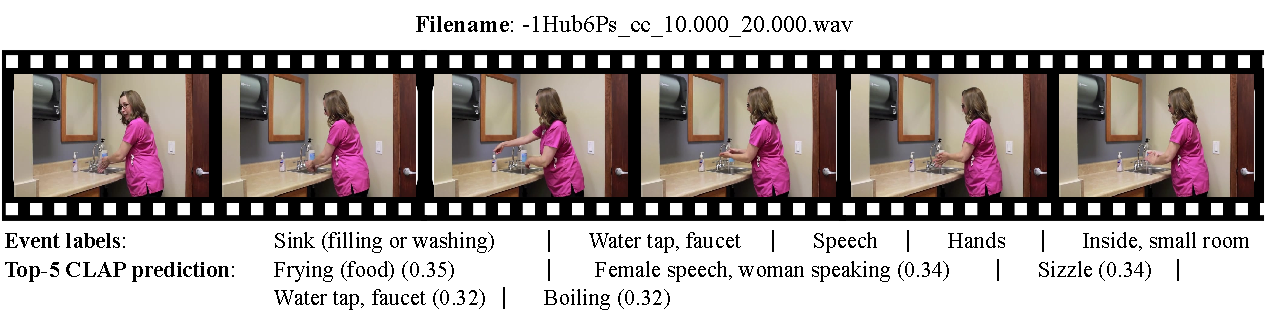
\includegraphics[width=\linewidth]{figs/AudioSet_femalespeech_6frame.pdf}
    \caption{An example of annotation errors in AudioSet. A woman is speaking in the audio clip while the corresponding event ``Female speech, woman speaking'' is not annotated.}
    \label{fig:audioset_missing_label}
\end{figure*}

\subsubsection{Zero-shot Transfer}
We first perform zero-shot inference on several datasets to reveal the transferring ability of CLAP.
Previous works enabling zero-shot inference, including AudioCLIP, Wav2CLIP and VIP$\sim$A$_\text{N}$T, are incorporated for comparison.
In these works, CLIP are incorporated for synthetic audio-text data generation or pre-training.
AudioCLIP is trained on AudioSet with audio event labels while Wav2CLIP is trained on VGGSound without using labels.
VIP$\sim$A$_\text{N}$T takes a similar pre-training scheme as CLAP: training on synthetic data first and then fine-tuning on real data.
We also include current SOTA results as topline for reference.
Results are shown in the upper half of \Cref{tab:classify_performance}.
On both ESC50 and UrbanSound8K, under the setting that AudioSet or AudioCaps are incorporated into pre-training, CLAP significantly outperforms AudioCLIP and VIP$\sim$A$_\text{N}$T.
On VGGSound, we list mAP in the parentheses to compare with Wav2CLIP.
CLAP outperforms Wav2CLIP even though the latter is pre-trained on the same dataset, indicating the effective transfer ability of CLAP.
However, CLAP achieves a very low mAP on AudioSet even though $\text{Enc}_A$ is trained on AudioSet before the contrastive pre-training.
Apart from the data distribution bias caused by the creation of AudioCaps (see \Cref{subsec:syn_data_generation}), we observe that the noise in AudioSet labels exacerbates the problem.
Previous works find that the annotation errors that not annotating events present in an audio clip are common in AudioSet~\cite{gong2021psla}.
An example is shown in \Cref{fig:audioset_missing_label}.
Speech from a woman can be clearly heard in the audio clip and CLAP assigns high probability to the event ``Female speech, woman speaking''.
However, the event does not occur in the AudioSet annotation.
We assume such annotation errors make the results of certain audio event classes not reliable.
On FSD50K where annotations are more reliable, CLAP achieves a much higher mAP.

%TODO awkward thing: current CLAP performs better without prompt。。。。。。




\subsubsection{Audio Encoder Fine-tuning}
Besides zero-shot inference, we also evaluate the transferring ability of CLAP by fine-tuning $\text{Enc}_A$ on these audio classification tasks.
We compare it with PANNs since they share the same CNN14 architecture.
The lower half of \Cref{tab:classify_performance} shows the results.
In both linear probing and fine-tuning settings, CLAP outperforms PANNs on ESC50 and TAU2019.
With only one FC layer as the classifier, the performance of linear probing CLAP on ESC50 and UrbanSound8K is even close to current SOTA results, indicating that CLAP serves as a powerful audio feature extractor.
Especially for small audio event datasets, CLAP is able to extract highly discriminative features for classification.


\section{Conclusion}

In this work, we propose an AudioSet tag-guided audio captioning model to generate large-scale parallel audio-text data on AudioSet.
The audio-text data generation approach does not incorporate CLIP to eliminate the noise induced from the visual modality. 
Based on the large-scale synthetic parallel audio-text data, we pre-train a bi-encoder audio-text model using contrastive learning.
After pre-training the model on the synthetic data and the real data successively, we obtain CLAP which can be transferred to a series of downstream tasks.
Experimental results on both cross-modal and single-modality tasks, including retrieval, generation and classification, validate the effectiveness of CLAP.
Under the difficult zero-shot condition that no training data are available, CLAP exhibits the state-of-the-art performance on most datasets. 

\section{Acknowledgements}
This work has been supported by National Natural Science Foundation of China (No.61901265), State Key Laboratory of Media Convergence Production Technology and Systems Project (No.SKLMCPTS\\2020003) and Shanghai Municipal Science and Technology Major Project (2021SHZDZX0102).
Experiments have been carried out on the PI supercomputer at Shanghai Jiao Tong University.


\bibliographystyle{ACM-Reference-Format}
\bibliography{refs}

\end{document}
\endinput
%%
%% End of file `sample-sigconf.tex'.
